\section{Game Design}
\label{sec:game_design}

This chapter covers our game design in regard to game play and the educational aspect.

\subsection{General Concept}
\label{sec:game_design:subsec:general_concept}

Our game design evolves from the idea of a serious game utilizing augmented reality techniques available on larger mobile devices, i.e.\ tablets or phones with a display size of at least 7 inch.
The educational goal is to convey knowledge about Celtic runes and culture through an engaging and entertaining game experience.
Learning is supported by a connection between the matter and the game mechanic, so the player improves his skill in the game by mastering knowledge about runes and vice versa.

The game is designed as a classical Tower Defense (TD) game. Players build towers to defend their city from increasingly difficult hordes of enemies.
This is explained in more detail in Section~\ref{sec:game_design:subsec:tower_defense}.
We use augmented reality to give the player control over the towers and buildings with printed physical markers, our `rune markers' (cf. Section~\ref{sec:game_design:subsec:runes}).
This is meant to increase the learning success by bringing the runes into focus while providing a refreshing game experience through novel control mechanics.
Knowledge about runes and Celtic history is presented gradually using a game campaign, where the player unlocks new runes and additionally information after increasingly more difficult levels. This is thoroughly explained in Section~\ref{sec:game_design:subsec:campaign}.

Finally we based the style of the game on available historical data about Celtic cities, defenses and enemies, which is covered in Section~\ref{sec:game_design:subsec:history}.

\subsection{Runes and Rune Markers}
\label{sec:game_design:subsec:runes}

As the primary goal of playing the game is to learn about Celtic runes, the runes are the core of our game experience.
Therefore we split the game into two distinct phases:
A preparation phase where the player interacts with physical representations of the runes, our rune markers, and a game phase where the player interacts with the augmented reality device.

\begin{wrapfigure}{R}{0.38\textwidth}
	\centering
	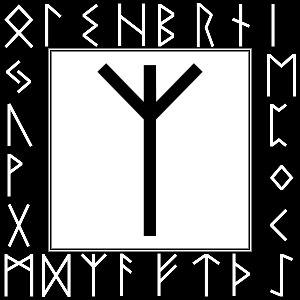
\includegraphics[width=0.35\textwidth]{figures/algiz0.jpeg}
	\caption{\label{fig:rune-marker} An Algiz rune marker for building towers}
\end{wrapfigure}

Our rune markers are printed out representations of runes that each have a unique effect in the game and need to be properly positioned by the player. Figure~\ref{fig:rune-marker} shows a rune marker for the \textit{`Algiz'} rune, which is used to build and position towers in-game.
As a player can use some runes multiple times, the rune markers have an additional unique boarder that enables the augmented reality tracking to distinguish similar runes.

As the basis for our runes and rune markers we used the 24 runes of the \textit{`Elder Futhark'}~\cite{elder-futhark}, the oldest form of the runic alphabets.
Almost\footnotemark all of the 24 runes have a special meaning in the game that closely relates to their original meaning.
For example the Algiz rune has the meanings \textit{`Elk', `Protection', `Defense'}~\cite{algiz} and is used to build towers.
Though, it must be noted here though that runes can have multiple meanings and the meaning is not always absolutely clear.
Rieckhoff and Biel point out that there is not Celtic historiography, literature or religious writings.~\cite{rieckhoff-runes} The absence of a large basis of usage, makes interpreting runes especially difficult.
\footnotetext{Unfortunately, we had to skip some runes as there was no reasonable way of mapping the rune to an in-game functionality.}
A complete table of the runes we used, the original meaning we used as a basis and their usage in-game can be found in Appendix TODO.

To properly play the game a player must recognize a rune and it's function in-game.
The player has as much time as he needs to study, recognize and properly place the runes in the preparation phase.\footnotemark
In combination with the coverage of most runes in-game and a close relation of their traditional meaning to the in-game usage, this measures support the learning success of the player.

\footnotetext{Though this can help him learn the runes, this was also a necessity due to the nature of augmented reality on a tablet computer.}

\subsection{Tower Defense}
\label{sec:game_design:subsec:tower_defense}

We use the basic and popular tower defense concepts for our core gameplay mechanics. Towers are manually placed on the map (through the position of the rune markers relative to the augmented reality map) and shoot incoming waves of enemies. The enemies have to be killed before they can reach the village, which is positioned with the \textit{`Mannaz'} rune marker and the anchor point of the augmented reality map.
If enemies reach the village, players loose health. When health reaches zero, the game is lost and the player has to start over.

Players can upgrade their towers by placing buff runes close to their tower rune. For example the \textit{`Kenaz'} rune adds fire damage to the tower it's linked to.
Additionally players can earn gold by building farms and harvesting them during the game phase, which adds additional interactivity to the game phase.
The gold can be used to buy additional lives during the preparation phase.

Although we would've liked to implemented additional mechanics, because of the difficulties encountered (cf. Section~\ref{sec:problems}), we decided to stick with this basic tower defense principle, which works with our augmented reality setup and is intuitive to use.


\subsection{Campaign}
\label{sec:game_design:subsec:campaign}

Because of the sheer number of runes the player has to learn before he is able to actually play the game, we slowly introduce the runes step by step in a campaign/ tutorial mode. That way, no one is overwhelmed by too many different rune symbols, their meanings and their meanings in-game, but is able to learn in small manageable steps. \\
After playing the campaign, a free-play mode is unlocked to offer a challenge for more experienced players without playing the campaign again. \\

\subsection{History}
\label{sec:game_design:subsec:history}


Manching nachempfunden

